\section{はじめに}

\section{問題}

この文章は、論文などを見ても数式の細かいところが分からないgraph-based SLAMについて、実際の計算方法を細かく解説するためのものです。

\subsection{ロボットの姿勢と座標系}

世界座標系$\Sigma_\text{w}$におけるロボットの姿勢(位置と向き)を
\begin{align}
	\V{x} =
	\begin{bmatrix}
		x \\ y \\ \theta
	\end{bmatrix}
\end{align}
で表す。また、$[x,y]^T$を原点として、$X$軸が世界座標系で$\theta$の方向を向いているロボット座標系
$\Sigma_\text{r}$を考える。これらの関係を図\ref{fig:coordinate}に示す。

\begin{figure}[h]
	\begin{center}
		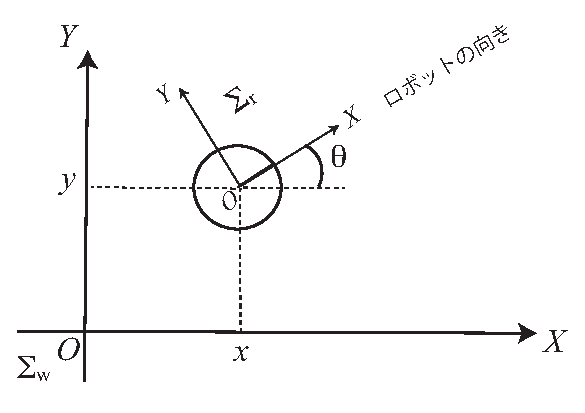
\includegraphics[width=0.5\linewidth]{./figs/coordinate.eps}
		\caption{世界座標系とロボットの姿勢}
		\label{fig:coordinate}
	\end{center}
\end{figure}
